\begin{frame}
  \frametitle{What is \textbf{mpi4py}?}
  \begin{itemize}
  \item Full-featured Python bindings for
    \href{http://www.mpi-forum.org}{\textbf{MPI}}.
  \item API based on the standard MPI-2 \Cpp bindings.
  \item Almost all MPI calls are supported.
    \begin{itemize}
    \item targeted to MPI-3 implementations.
    \item also works with MPI-1/2 implementations.
    \end{itemize}
  \end{itemize}
\end{frame}

\begin{frame}
  \frametitle{Implementation}
  Implemented with \href{http://www.cython.org}{\textbf{Cython}}
  \begin{itemize}
  \item Code base far easier to write, maintain, and extend.
  \item Faster than other solutions (mixed Python and C codes).
  \item \textsl{Pythonic} APIs that runs at C speed !
  \end{itemize}
\end{frame}

\begin{frame}
  \frametitle{Implementation - Cython [1]}
  \footnotesize
  \inputminted[firstline=1]{cython}{cython-mpi4py.pxi}
\end{frame}

\begin{frame}
  \frametitle{Implementation - Cython [2]}
  \footnotesize
  \inputminted[firstline=3]{cython}{cython-mpi4py.pyx}
\end{frame}

\begin{frame}
  \frametitle{Features -- MPI-1}
  \begin{itemize}
  \item Process groups and communication domains.
    \begin{itemize}
    \item intracommunicators
    \item intercommunicators
    \end{itemize}
  \item Point to point communication.
    \begin{itemize}
    \item blocking (send/recv)
    \item nonblocking (isend/irecv + test/wait)
    \end{itemize}
  \item Collective operations.
    \begin{itemize}
    \item synchronization (barrier)
    \item communication (broadcast, scatter/gather)
    \item global reductions (reduce, scan)
    \end{itemize}
  \end{itemize}
\end{frame}

% \begin{frame}
%   \frametitle{Features -- MPI-2}
%   \begin{itemize}
%   \item Extended collective operations (intercommunicators).
%   \item Dynamic process management (spawn, connect/accept).
%   \item Parallel I/O (read/write).
%   \item One-sided operations, a.k.a. RMA (put/get/accumulate).
%   \end{itemize}
% \end{frame}

% \begin{frame}
%   \frametitle{Features -- MPI-3}
%   \begin{itemize}
%   \item Matched point to point communication (mprobe).
%   \item Nonbloking collective operations (ibarrier, ibcast, etc.).
%   \item Neighborhood collective operations (neighbor allgather/toall).
%   \item Extended RMA support (shared memory).
%   \end{itemize}
% \end{frame}

\begin{frame}
  \frametitle{Features -- Python}
  \begin{itemize}
  \item Communication of Python objects.
    \begin{itemize}
    \item high level and very convenient, based in \texttt{pickle}
      serialization
    \item can be slow for large data (CPU and memory consuming)
    \end{itemize}
    \fbox{\texttt{send(object)}}\\
    \fbox{%
      \texttt{object} $\longrightarrow{}$%
      \texttt{pickle.dump()} $\longrightarrow{}$%
      \texttt{MPI\_Send()}
    }
    \\\hspace{39ex}\\
    \fbox{\texttt{object = recv()}}
    \fbox{%
      \texttt{object} $\longleftarrow{}$%
      \texttt{pickle.load()} $\longleftarrow{}$%
      \texttt{MPI\_Recv()}}
  \item Communication of array data
    (e.g. \href{http://numpy.scipy.org}{\textbf{NumPy}} arrays).
    \begin{itemize}
    \item lower level, slightly more verbose
    \item very fast, almost C speed (for messages above 5-10 KB)
    \end{itemize}
    \fbox{message = \texttt{[object, (count, displ), datatype]}}
  \end{itemize}
\end{frame}

\begin{frame}
  \begin{center}
    Point to Point Throughput -- Gigabit Ethernet
  \end{center}
  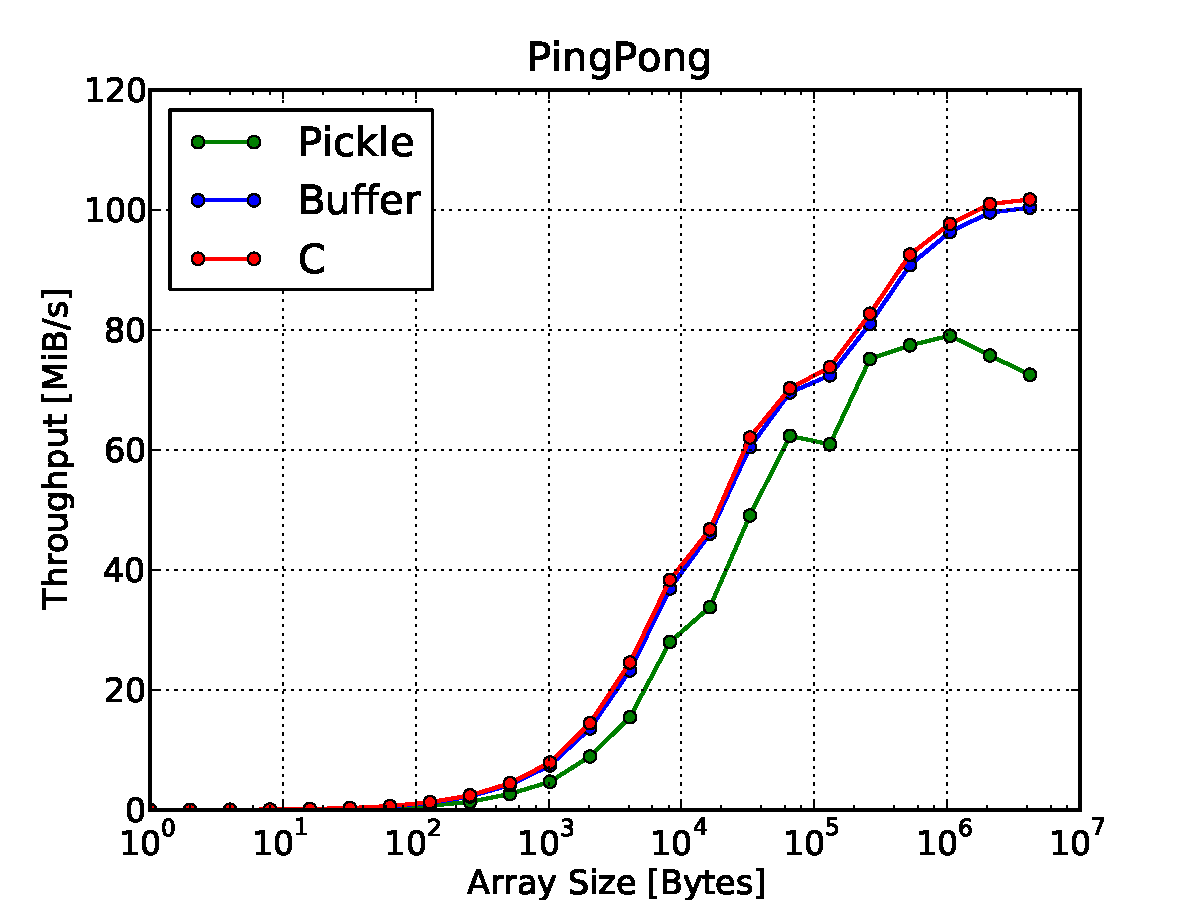
\includegraphics[scale=0.5]{PingPong_GE.pdf}
\end{frame}
\begin{frame}
  \begin{center}
    Point to Point Throughput -- Shared Memory
  \end{center}
  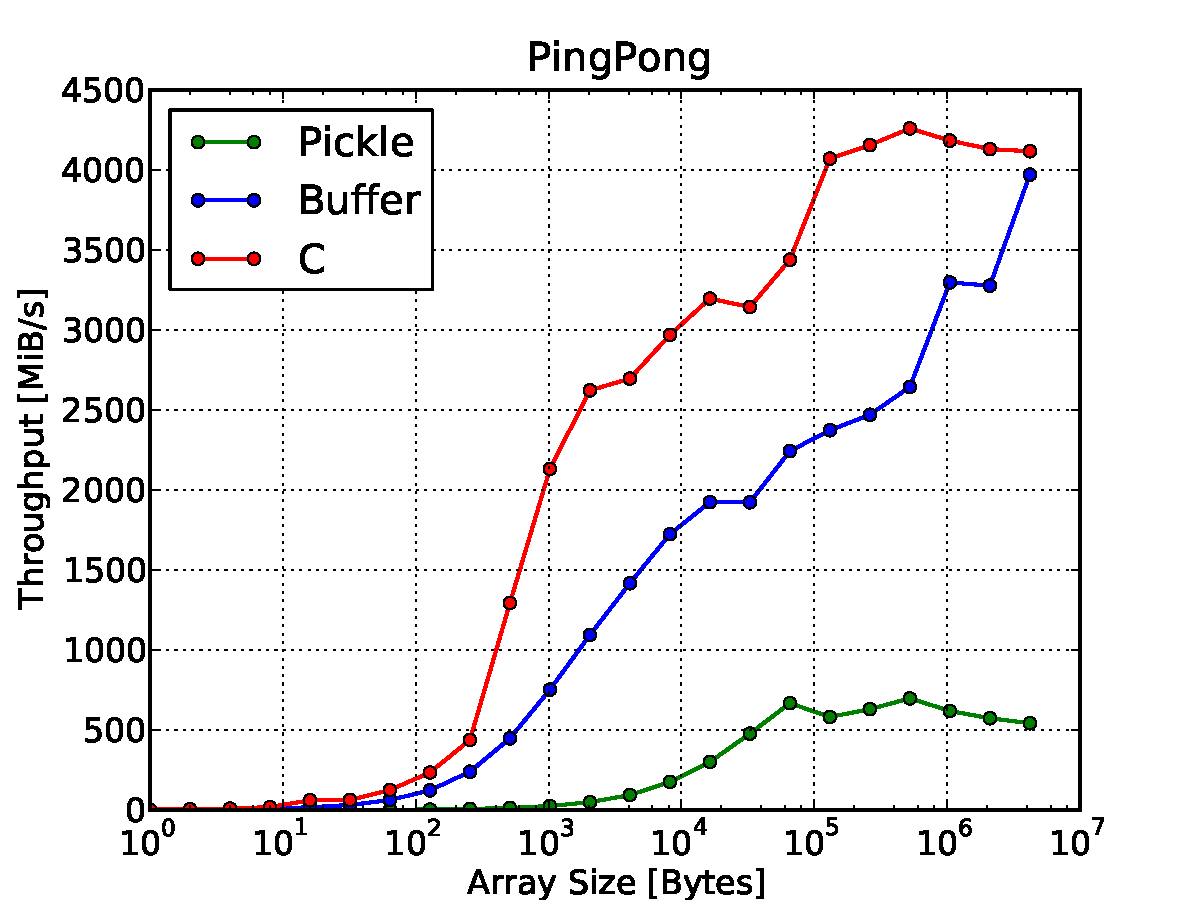
\includegraphics[scale=0.5]{PingPong_SM.pdf}
\end{frame}

\begin{frame}[fragile]
  \frametitle{Features -- IPython}
  Integration with \href{http://ipython.scipy.org}{\textbf{IPython}}
  enables MPI to be used \emph{interactively}.
  \begin{itemize}
  \item Start engines with MPI enabled
\begin{verbatim}
   $ ipcluster start -n 16 --engines=MPI
\end{verbatim}
  \item Connect to the engines
\begin{verbatim}
   $ ipython
   In [1]: from ipyparallel import Client
   In [2]: rc = Client()
\end{verbatim}
  \item Execute commands using \texttt{\%px}
\begin{verbatim}
   In [4]: %px from mpi4py import MPI
   In [5]: %px print(MPI.Get_processor_name())
\end{verbatim}
  \end{itemize}
\end{frame}

% \begin{frame}
%   \frametitle{Features -- Interoperability}
%   Support for wrapping MPI-based libraries.
%   \begin{itemize}
%   \item You can use \href{http://cython.org}{\textbf{Cython}}
%     (\texttt{cimport} statement).
%   \item You can use \href{http://swig.org}{\textbf{SWIG}}
%     (\textsl{typemaps} provided).
%   \item You can use \href{http://f2py.com}{\textbf{F2Py}}
%     (\texttt{py2f()}/\texttt{f2py()} methods).
%   \item You can use
%     \href{http://www.boost.org}{\textbf{Boost::Python}} or
%     \textbf{hand-written C} extensions.
%   \end{itemize}
%   \textbf{mpi4py} allows using virtually any MPI-based
%   C/\Cpp/Fortran library code from Python.
% \end{frame}
